\documentclass[compress, aspectratio=169]{beamer}

\usefonttheme{professionalfonts}

\usepackage{fontspec}
\usepackage{polyglossia}
\setmainlanguage{german}

\usepackage{mathtools}
\usepackage[
  math-style=ISO,
  bold-style=ISO,
  nabla=upright,
  partial=upright,
]{unicode-math}

\usepackage[locale=DE, math-rm=\mathup]{siunitx}

\usepackage{graphicx}

\usepackage{tikz}
\usetikzlibrary{arrows}
\usetikzlibrary{arrows.meta}

\usepackage{pgfplots}
\usepgfplotslibrary{polar}
\pgfplotsset{compat=1.12}


% \usepackage{xfrac}

\newcommand\SIQ[2]{\ensuremath{#1\mathrel{/}\si{#2}}}

\usetheme{vertex}


\author{Maximilian Nöthe}
\date[21.5.2015]{Seminar Radioastronomie, TU Dortmund, 21.5.2015}
\title{Das Wasserstoffspektrum}
\subtitle{in der Radioastronomie}

\begin{document}
\maketitle


\begin{frame}{Die \SI{21}{\centi\meter}-Linie}
  \begin{columns}[c]%
    \begin{column}{0.6\textwidth}%
      \begin{tikzpicture}[
    level/.style={very thick},
  photon/.style={-{Stealth[length=2mm]}, thick, decorate, decoration={snake, pre length=1mm, post length=2mm,}}, connect/.style={dashed, very thick},
  ]
  \draw[level] (0, 0) -- (+1.5, 0) node at (0, 0) [above] {$1^2S_{\sfrac{1}{2}}$};
  \draw[connect] (1.5, 0) -- +(1.5,  1);
  \draw[connect] (1.5, 0) -- +(1.5, -1);
  \draw[level] (3,  1) -- +(1.5, 0);
  \draw[level] (3, -1) -- +(1.5, 0);

  \draw[red!70!black, ->, thick] (3.75, 1) -- +(0, -2)
    node[right, midway] {$\increment E = \SI{5.9e-6}{\electronvolt}$};
  \draw[red!70!black, photon] (3.75, 0) -- + (-3, -2)
  node[below, align=left] {$λ = \SI{21.11}{\centi\meter}$ \\ $f = \SI{1420.406}{\mega\hertz}$};
  \node[] at (5,  1) {$\uparrow \quad \uparrow$};
  \node[] at (5, -1) {$\uparrow \quad \downarrow$};
  \node[] at (5,  1.5) {$\mathup{p}\quad\mathup{e}$};
\end{tikzpicture}

    \end{column}%
    \begin{column}{0.4\textwidth}%
      \begin{itemize}
        \item Hyperfeinstruktur-Übergang in neutralem H
        \item Einzige Möglichkeit Gaswolken zu vermessen
        \item stark unterdrückt
      \end{itemize}
    \end{column}%
  \end{columns}%
\end{frame}

\begin{frame}{Die \SI{21}{\centi\meter}-Linie – Vermessung der Milchstraße}%
  \begin{columns}[c]%
    \begin{column}{0.5\textwidth}%
      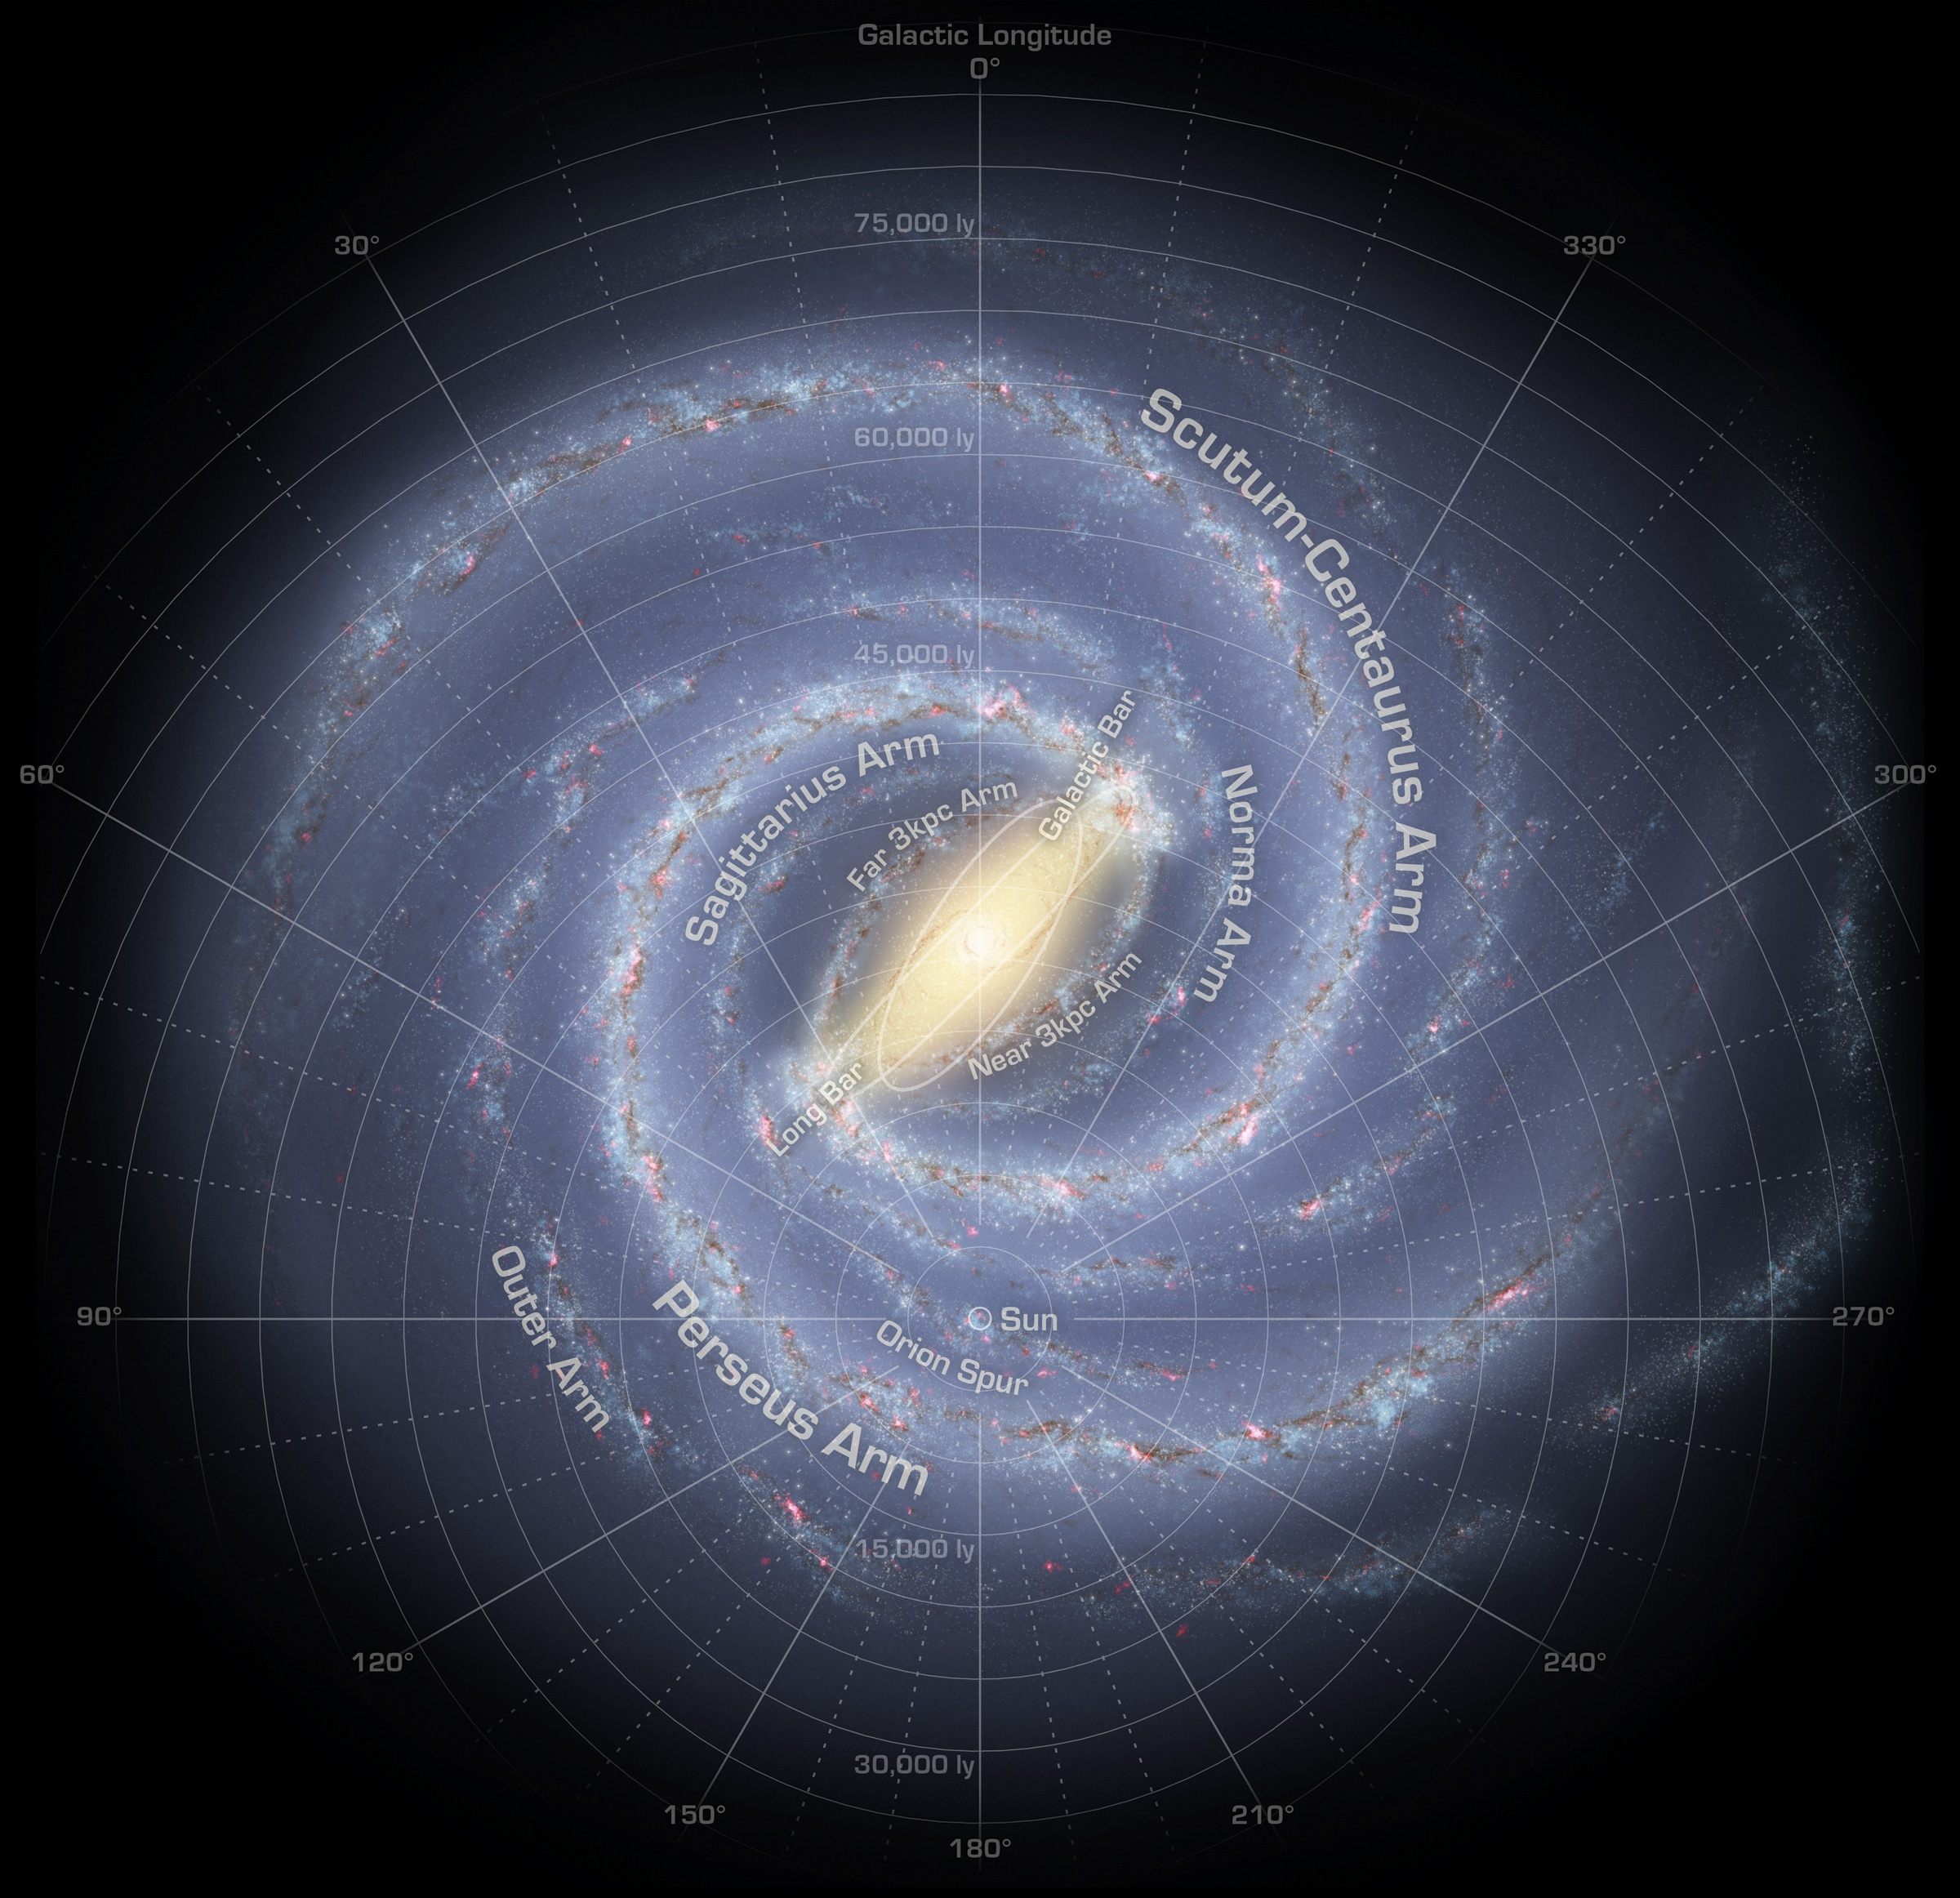
\includegraphics[width=\textwidth]{images/milkyway_structure_big_crop.jpeg}
    \end{column}%
    \begin{column}{0.5\textwidth}%
      \only<1>{%
      \begin{tikzpicture}[overlay, remember picture, shift={(current page.center)}]%
        \draw[red!70!black, thick, o->] (-3.895, -1.52) -- +(55:5);%
      \end{tikzpicture}%
      \begin{tikzpicture}%
        \begin{axis}[%
            title={$T_b$ für $l=\SI{335}{\degree}$},
            xmin=21.09,
            xmax=21.12,
            ymin=-10,
            ymax=120,
            width=\textwidth,
            xlabel={\SIQ{λ}{\centi\meter}},
            ylabel={$\SIQ{T_b}{\kelvin}$},
          ]%
          \addplot[red!70!black] table[x index=3, y index=1]{./data/radial_velocity_l335.txt};%
        \end{axis}%
      }%
      \only<2>{%
      \begin{tikzpicture}[overlay, remember picture, shift={(current page.center)}]%
        \draw[red!70!black, thick, o->] (-3.935, -1.44) -- +(0:4);
      \end{tikzpicture}%
      \begin{tikzpicture}%
        \begin{axis}[
            title={$T_b$ für $l=\SI{270}{\degree}$},
            xmin=21.09,
            xmax=21.12,
            ymin=-10,
            ymax=120,
            width=\textwidth,
            xlabel={\SIQ{λ}{\centi\meter}},
            ylabel={$\SIQ{T_b}{\kelvin} $},
          ]%
          \addplot[red!70!black] table[x index=3, y index=1]{./data/radial_velocity_l270.txt};%
        \end{axis}%
      }%
      \end{tikzpicture}%
    \end{column}%
  \end{columns}%
\end{frame}
\end{document}
